\section{How CrashSimulator Works}
\label{SEC:approach}

\begin{figure}[t]
  \center{}
  \fbox{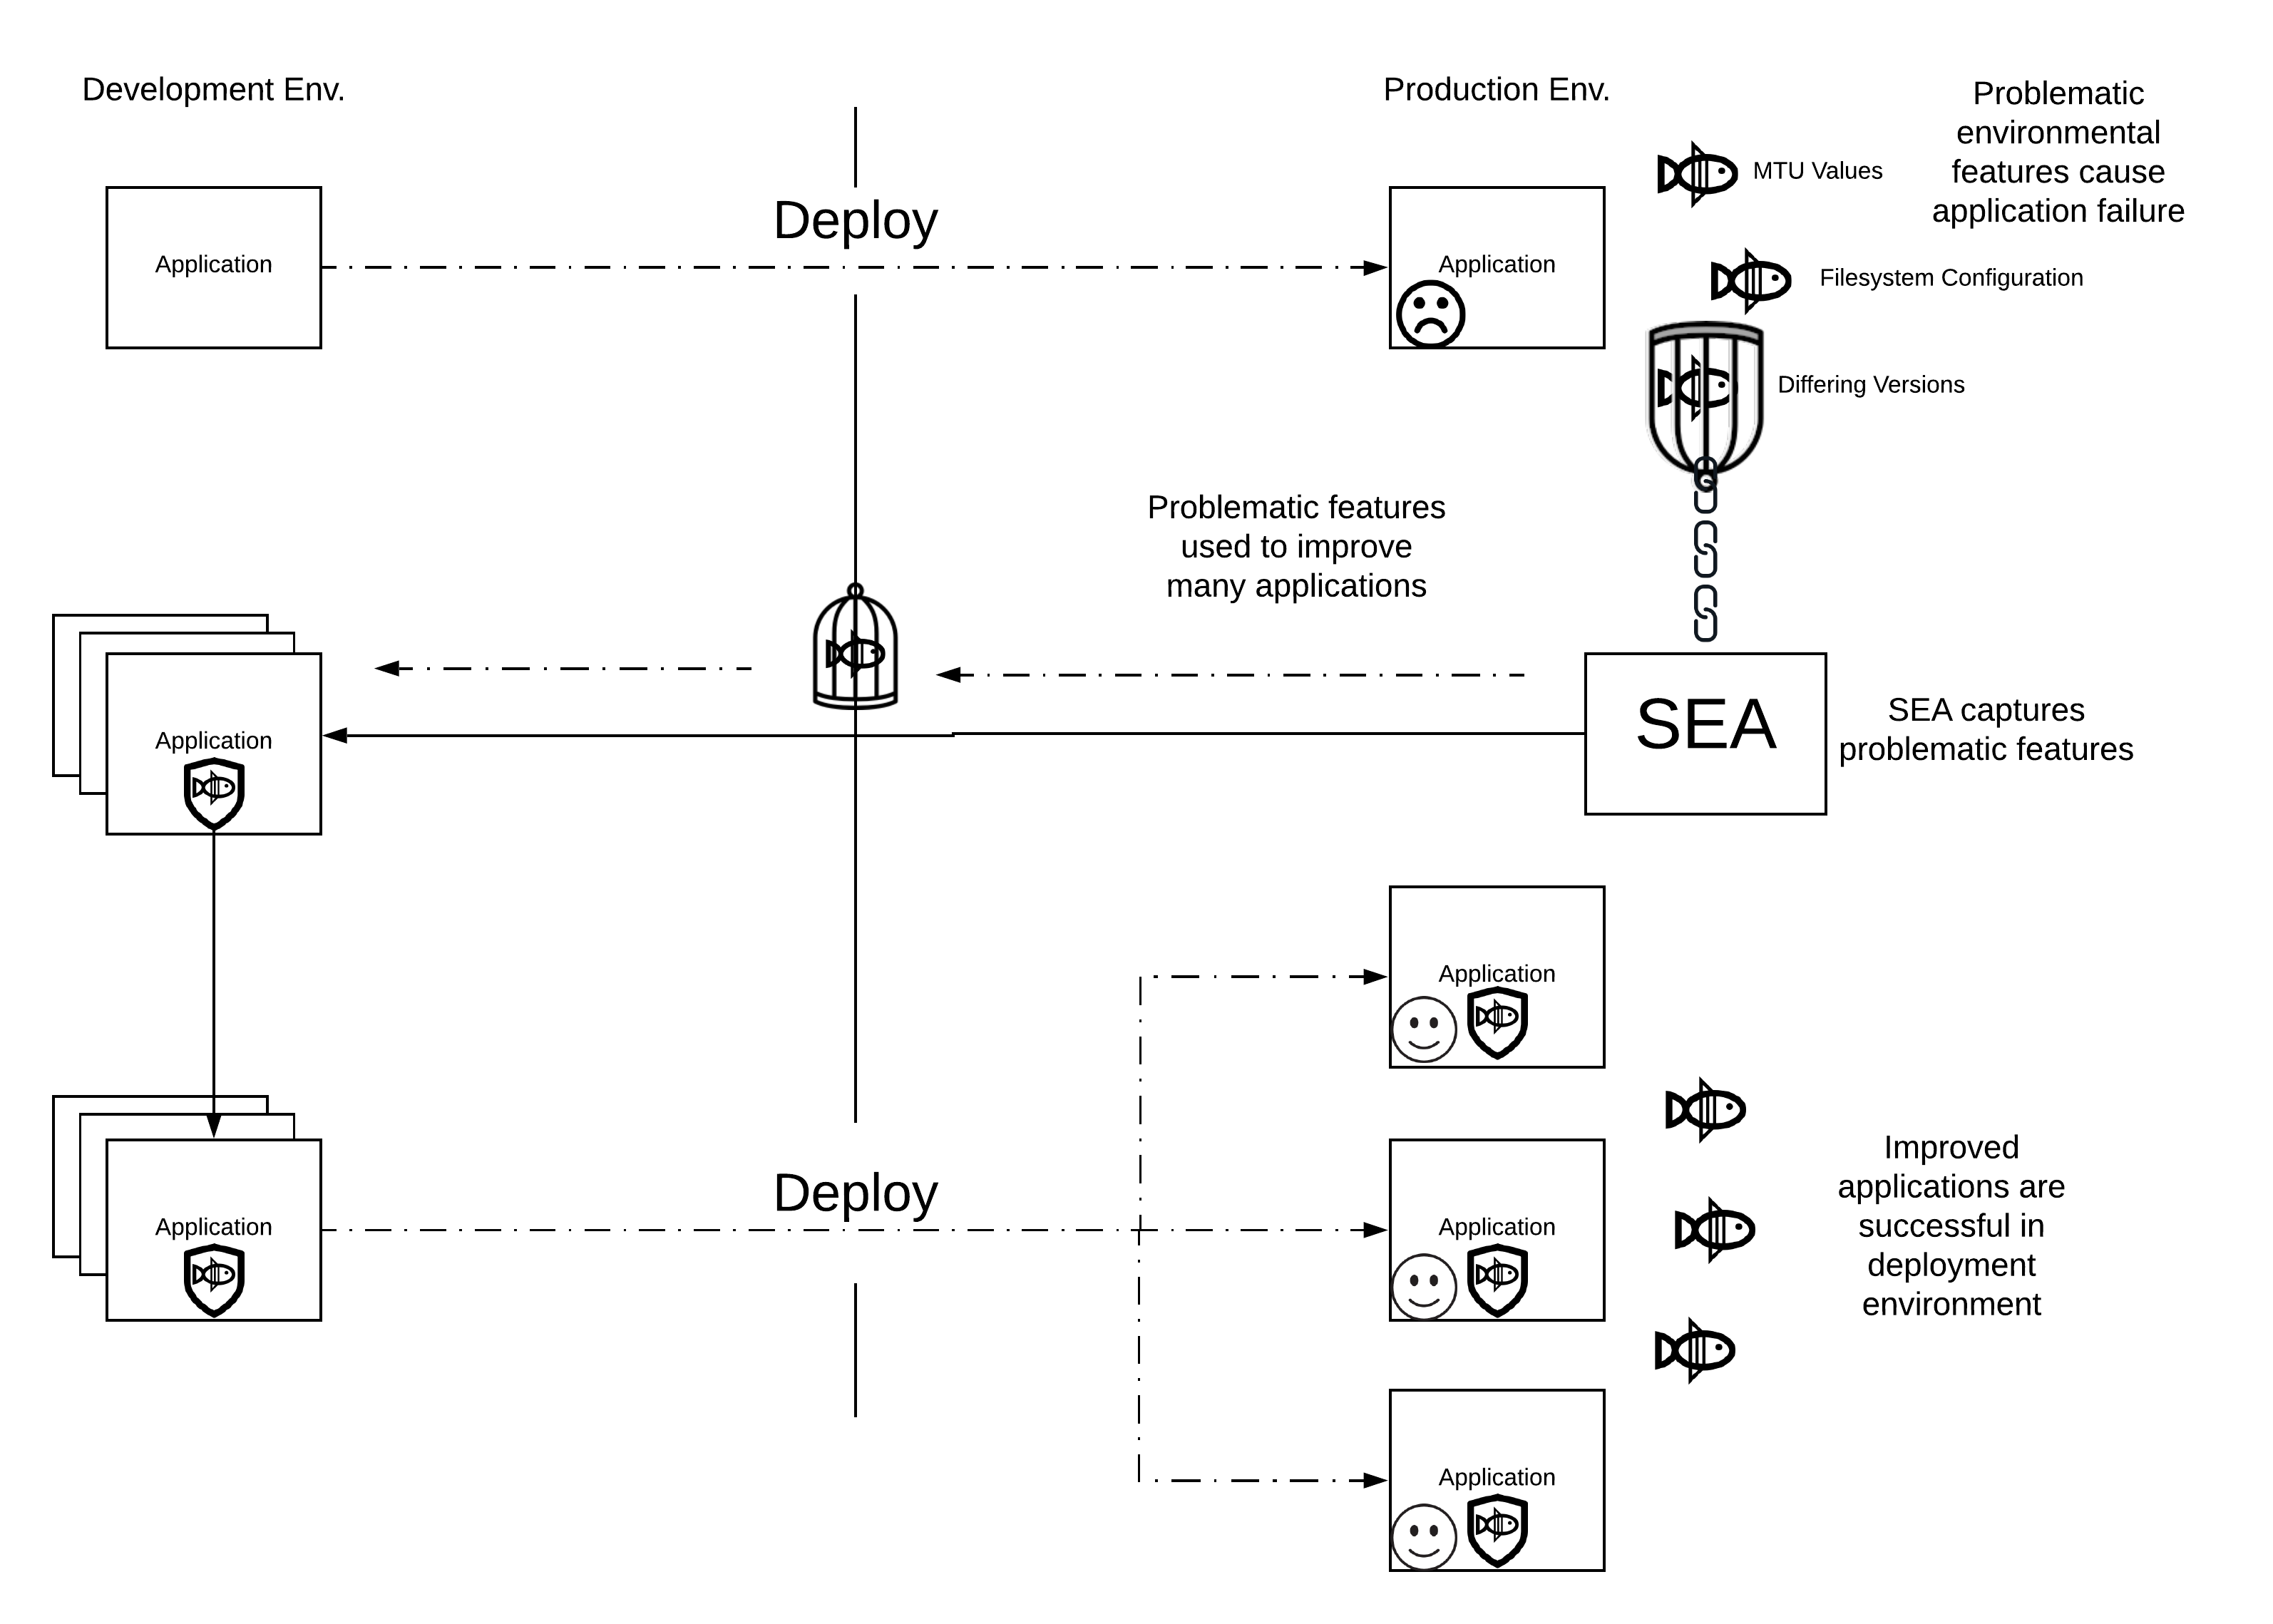
\includegraphics[scale=.5]{images/approach}}
  \caption{Diagram illustrating CrashSimulator's approach}
  \label{figure:approach}
\end{figure}

Included with CrashSimulator is a corpus of environmental anomalies
that we found to be problematic for real world
applications.
From a user's perspective, using CrashSimulator boils down to selecting one
of the supplied anomalies to test an application against and allowing the
tool to take over.  Behind the scenes,
CrashSimulator uses a four-step operation to identify bugs resulting from
the chosen anomaly.
These steps, illustrated in Figure~\ref{figure:approach} are as follows.
First, CrashSimulator records the application being tested.  Next, it
modifies this recording so that the chosen anomaly is present.
Finally, It then replays this
modified recording, exposing the application to the chosen anomaly.

\subsection{Trace Recording and Anomaly Injection}

Before testing can begin
CrashSimulator generates recording of the application to be
tested as it executes in an environment where the chosen anomaly is not
present.  This recording acts both as a medium into which anomalies can be
injected and a log of the application's behavior under normal
conditions.  Once this recording is complete CrashSimulator runs a script,
known as a mutator, associated with the chosen anomaly.
This script is responsible for identifying
the points in the recording
where the anomaly can be injected and modifying
the recording such that the anomaly is present.

Once this mutated recording has been generated, CrashSimulator replays the
application using this recording.
Because replaying the
recording faithfully follows the described system call behavior, the
application is exposed to the injected
anomalous conditions.  For
example, suppose an anomaly causes a call to {\tt read()} to fail with
return value of -1 and {\tt errno} set to {\tt EINVAL}.  Exposing an
application to this situation only requires modifying the recording,
such that this read call reflects the above values.

We refer to this process as {\tt Result Based Simulation} and it is based
on the idea that environmental anomalies will be present in the results of
the procedure calls an application makes that are influenced by the
applications environment.
This technique could be carried out several different levels
of execution.  For example, the results of calls to functions in a
platform's {\tt libc} library could be intercepted and modified to reflect
environmental differences.  At a higher level, virtual machines like the
{\tt JVM} could be adapted to allow the results and side effects of calls
to be interposed upon in a similar fashion.
For CrashSimulator's purposes we chose to interpose
on the results and side effects of system calls in order to simulate
unusual environment.  Operating at this level provides a few key
advantages.  First, there is already robust tooling in the Linux kernel
that allows for the interception and modification of system call results
and side effects.  Additionally, Linux system call semantics are well
defined which simplifies implementation.  Finally, operating at this level
allows CrashSimulator to test applications written any language that can
execute Linux system calls.

\subsection{Analyzing an Execution}

After an application has been exposed to an anomaly CrashSimulator must
make a determination about whether the application may be responding to it.
This determination comes down to whether or not
the application alters its
system call behavior.  When an anomalous
behavior is injected into a replay execution,
it is expected that the application under
test will deal with it in some way.  For example, applications can
be expected to behave differently when the structure returned by a call to
{\tt stat()} indicates the target file is a block device,
rather than a regular
file.  CrashSimulator bases its assessment on the assumption that the way
an
application deals with the anomaly will yield
different program paths (and therefore different system calls) than
those
executed when the original system call trace was recorded.
If the application
does not alter its behavior, it has not
correctly handled this flaw --- a failing result.  Alternatively, if the
application does deviate, it is likely that the application is taking some
action to handle the injected condition --- an indication of possibly
correct behavior.

This approach is often sufficient to classify application behavior.  As
with traditional tests, CrashSimulator does not tell us that an application
is bug free in a given situation; instead, it asserts that an application
has incorrectly handled a given situation.  In our experience, actually
exposing applications to anomalies CrashSimulator reported as unhandled
did result
in bugs ranging from simple hangs to more dramatic crashes that
had the side effect of consuming all available resources or filling
available disk space with garbage.
